\chapter{树算法}

\index{树}

\key{树}是一个连通的、无环的图，
由$n$个节点和$n-1$条边组成。
从树中移除任意一条边都会将其
分割为两个连通分量，
而在树中添加任意一条边都会产生一个环。
此外，树的任意两个节点之间
总存在唯一的路径。

例如，下面的树由8个节点和7条边组成：
\begin{center}
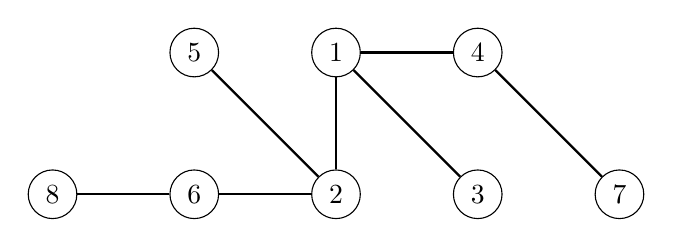
\begin{tikzpicture}[scale=0.9]
\node[draw, circle] (1) at (0,3) {$1$};
\node[draw, circle] (2) at (2,3) {$4$};
\node[draw, circle] (3) at (0,1) {$2$};
\node[draw, circle] (4) at (2,1) {$3$};
\node[draw, circle] (5) at (4,1) {$7$};
\node[draw, circle] (6) at (-2,3) {$5$};
\node[draw, circle] (7) at (-2,1) {$6$};
\node[draw, circle] (8) at (-4,1) {$8$};
\path[draw,thick,-] (1) -- (2);
\path[draw,thick,-] (1) -- (3);
\path[draw,thick,-] (1) -- (4);
\path[draw,thick,-] (2) -- (5);
\path[draw,thick,-] (3) -- (6);
\path[draw,thick,-] (3) -- (7);
\path[draw,thick,-] (7) -- (8);
\end{tikzpicture}
\end{center}

\index{叶子}

树的\key{叶子}是度数为1的节点，
即只有一个邻居的节点。
例如，上面那棵树的叶子
是节点3、5、7和8。

\index{根}
\index{有根树}

在\key{有根}树中，其中一个节点
被指定为树的\key{根}，
所有其他节点都
位于根的下方。
例如，在下面的树中，
节点1是根节点。

\begin{center}
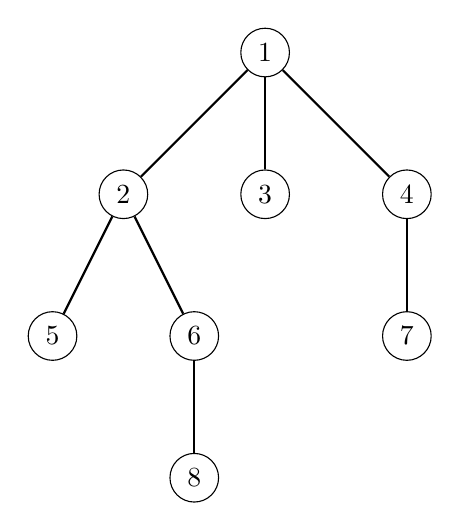
\begin{tikzpicture}[scale=0.9]
\node[draw, circle] (1) at (0,3) {$1$};
\node[draw, circle] (4) at (2,1) {$4$};
\node[draw, circle] (2) at (-2,1) {$2$};
\node[draw, circle] (3) at (0,1) {$3$};
\node[draw, circle] (7) at (2,-1) {$7$};
\node[draw, circle] (5) at (-3,-1) {$5$};
\node[draw, circle] (6) at (-1,-1) {$6$};
\node[draw, circle] (8) at (-1,-3) {$8$};
\path[draw,thick,-] (1) -- (2);
\path[draw,thick,-] (1) -- (3);
\path[draw,thick,-] (1) -- (4);
\path[draw,thick,-] (2) -- (5);
\path[draw,thick,-] (2) -- (6);
\path[draw,thick,-] (4) -- (7);
\path[draw,thick,-] (6) -- (8);
\end{tikzpicture}
\end{center}
\index{子节点}
\index{父节点}

在有根树中，一个节点的\key{子节点}
是它下方的邻居，而一个节点的\key{父节点}
是它上方的邻居。
每个节点恰好有一个父节点，
除了根节点没有父节点。
例如，在上面的树中，
节点2的子节点是节点5和6，
其父节点是节点1。

\index{子树}

有根树的结构是\emph{递归的}：
树的每个节点作为一个\key{子树}的根，
该子树包含节点本身以及
其子节点的子树中的所有节点。
例如，在上面的树中，节点2的子树
由节点2、5、6和8组成：
\begin{center}
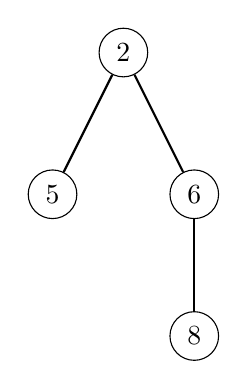
\begin{tikzpicture}[scale=0.9]
\node[draw, circle] (2) at (-2,1) {$2$};
\node[draw, circle] (5) at (-3,-1) {$5$};
\node[draw, circle] (6) at (-1,-1) {$6$};
\node[draw, circle] (8) at (-1,-3) {$8$};
\path[draw,thick,-] (2) -- (5);
\path[draw,thick,-] (2) -- (6);
\path[draw,thick,-] (6) -- (8);
\end{tikzpicture}
\end{center}

\section{树遍历}

通用的图遍历算法
可以用来遍历树的节点。
然而，树的遍历比一般图的遍历更容易实现，因为
树中没有环，不可能
从多个方向到达一个节点。

遍历树的典型方法是从
一个任意节点开始进行深度优先搜索。
可以使用以下递归函数：

\begin{lstlisting}
void dfs(int s, int e) {
    // 处理节点 s
    for (auto u : adj[s]) {
        if (u != e) dfs(u, s);
    }
}
\end{lstlisting}

该函数有两个参数：当前节点$s$
和前一个节点$e$。
参数$e$的作用是确保
搜索只移动到
尚未访问过的节点。

以下函数调用从
节点$x$开始搜索：

\begin{lstlisting}
dfs(x, 0);
\end{lstlisting}

在第一次调用中$e=0$，因为没有
前一个节点，所以可以
朝树中的任意方向前进。

\subsubsection{动态规划}

动态规划可以用来在树遍历过程中
计算一些信息。
例如，使用动态规划，我们可以在$O(n)$时间内
为有根树的每个节点计算
其子树中的节点数
或从该节点到叶子的最长路径长度。

作为示例，让我们为每个节点$s$计算
一个值$\texttt{count}[s]$：其子树中的节点数。
子树包含节点本身以及
其子节点的子树中的所有节点，
因此我们可以使用以下代码递归计算节点数：

\begin{lstlisting}
void dfs(int s, int e) {
    count[s] = 1;
    for (auto u : adj[s]) {
        if (u == e) continue;
        dfs(u, s);
        count[s] += count[u];
    }
}
\end{lstlisting}

\section{直径}

\index{直径}

树的\key{直径}
是两个节点之间路径的最大长度。
例如，考虑下面的树：
\begin{center}
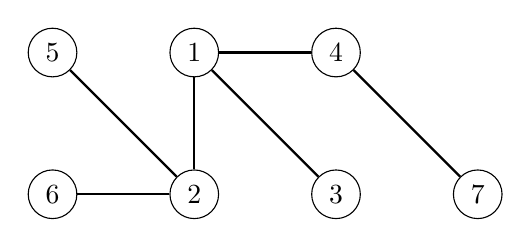
\begin{tikzpicture}[scale=0.9]
\node[draw, circle] (1) at (0,3) {$1$};
\node[draw, circle] (2) at (2,3) {$4$};
\node[draw, circle] (3) at (0,1) {$2$};
\node[draw, circle] (4) at (2,1) {$3$};
\node[draw, circle] (5) at (4,1) {$7$};
\node[draw, circle] (6) at (-2,3) {$5$};
\node[draw, circle] (7) at (-2,1) {$6$};
\path[draw,thick,-] (1) -- (2);
\path[draw,thick,-] (1) -- (3);
\path[draw,thick,-] (1) -- (4);
\path[draw,thick,-] (2) -- (5);
\path[draw,thick,-] (3) -- (6);
\path[draw,thick,-] (3) -- (7);
\end{tikzpicture}
\end{center}
这棵树的直径为4，
对应以下路径：
\begin{center}
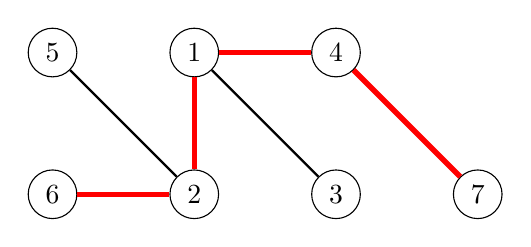
\begin{tikzpicture}[scale=0.9]
\node[draw, circle] (1) at (0,3) {$1$};
\node[draw, circle] (2) at (2,3) {$4$};
\node[draw, circle] (3) at (0,1) {$2$};
\node[draw, circle] (4) at (2,1) {$3$};
\node[draw, circle] (5) at (4,1) {$7$};
\node[draw, circle] (6) at (-2,3) {$5$};
\node[draw, circle] (7) at (-2,1) {$6$};
\path[draw,thick,-] (1) -- (2);
\path[draw,thick,-] (1) -- (3);
\path[draw,thick,-] (1) -- (4);
\path[draw,thick,-] (2) -- (5);
\path[draw,thick,-] (3) -- (6);
\path[draw,thick,-] (3) -- (7);

\path[draw,thick,-,color=red,line width=2pt] (7) -- (3);
\path[draw,thick,-,color=red,line width=2pt] (3) -- (1);
\path[draw,thick,-,color=red,line width=2pt] (1) -- (2);
\path[draw,thick,-,color=red,line width=2pt] (2) -- (5);
\end{tikzpicture}
\end{center}
注意，可能有多条最大长度的路径。
在上面的路径中，我们可以用节点5替换节点6，
从而得到另一条长度为4的路径。

接下来我们将讨论两种$O(n)$时间复杂度的算法
来计算树的直径。
第一种算法基于动态规划，
第二种算法使用两次深度优先搜索。

\subsubsection{算法1}

解决许多树问题的一种通用方法
是首先任意指定树的根。
之后，我们可以尝试对每个子树
分别解决问题。
我们计算直径的第一个算法
就是基于这个思想。

一个重要的观察是，有根树中的每条路径
都有一个\emph{最高点}：
即属于该路径的最高节点。
因此，我们可以为每个节点计算
以该节点为最高点的最长路径长度。
这些路径中的一条对应树的直径。

例如，在下面的树中，
节点1是对应直径的路径上的
最高点：
\begin{center}
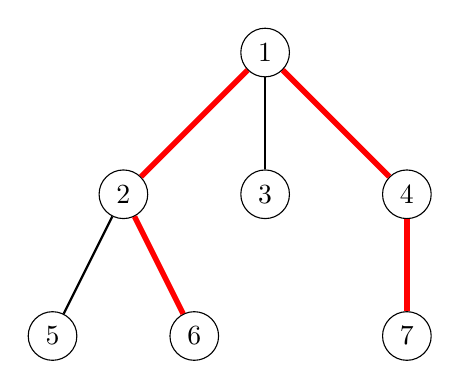
\begin{tikzpicture}[scale=0.9]
\node[draw, circle] (1) at (0,3) {$1$};
\node[draw, circle] (2) at (2,1) {$4$};
\node[draw, circle] (3) at (-2,1) {$2$};
\node[draw, circle] (4) at (0,1) {$3$};
\node[draw, circle] (5) at (2,-1) {$7$};
\node[draw, circle] (6) at (-3,-1) {$5$};
\node[draw, circle] (7) at (-1,-1) {$6$};
\path[draw,thick,-] (1) -- (2);
\path[draw,thick,-] (1) -- (3);
\path[draw,thick,-] (1) -- (4);
\path[draw,thick,-] (2) -- (5);
\path[draw,thick,-] (3) -- (6);
\path[draw,thick,-] (3) -- (7);

\path[draw,thick,-,color=red,line width=2pt] (7) -- (3);
\path[draw,thick,-,color=red,line width=2pt] (3) -- (1);
\path[draw,thick,-,color=red,line width=2pt] (1) -- (2);
\path[draw,thick,-,color=red,line width=2pt] (2) -- (5);
\end{tikzpicture}
\end{center}

我们为每个节点$x$计算两个值：
\begin{itemize}
\item $\texttt{toLeaf}(x)$：从$x$到任意叶子的路径的最大长度
\item $\texttt{maxLength}(x)$：最高点为$x$的路径的最大长度
\end{itemize}
例如，在上面的树中，
$\texttt{toLeaf}(1)=2$，因为存在路径
$1 \rightarrow 2 \rightarrow 6$，
而$\texttt{maxLength}(1)=4$，
因为存在路径
$6 \rightarrow 2 \rightarrow 1 \rightarrow 4 \rightarrow 7$。
在这种情况下，$\texttt{maxLength}(1)$等于直径。

可以使用动态规划在$O(n)$时间内
计算所有节点的上述值。
首先，计算$\texttt{toLeaf}(x)$时，
我们遍历$x$的子节点，
选择$\texttt{toLeaf}(c)$最大的子节点$c$，
然后给该值加一。
然后，计算$\texttt{maxLength}(x)$时，
我们选择两个不同的子节点$a$和$b$，
使得$\texttt{toLeaf}(a)+\texttt{toLeaf}(b)$
之和最大，然后给该和加二。

\subsubsection{算法2}

另一种计算树直径的高效方法
基于两次深度优先搜索。
首先，我们在树中选择一个任意节点$a$，
并找到距离$a$最远的节点$b$。
然后，我们找到距离$b$最远的节点$c$。
树的直径就是$b$和$c$之间的距离。

在下面的图中，$a$、$b$和$c$可以是：
\begin{center}
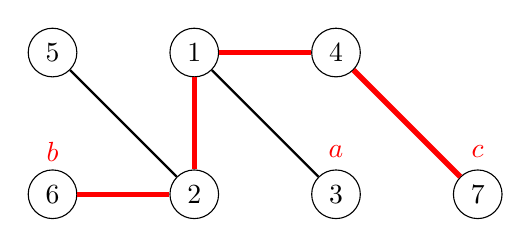
\begin{tikzpicture}[scale=0.9]
\node[draw, circle] (1) at (0,3) {$1$};
\node[draw, circle] (2) at (2,3) {$4$};
\node[draw, circle] (3) at (0,1) {$2$};
\node[draw, circle] (4) at (2,1) {$3$};
\node[draw, circle] (5) at (4,1) {$7$};
\node[draw, circle] (6) at (-2,3) {$5$};
\node[draw, circle] (7) at (-2,1) {$6$};
\path[draw,thick,-] (1) -- (2);
\path[draw,thick,-] (1) -- (3);
\path[draw,thick,-] (1) -- (4);
\path[draw,thick,-] (2) -- (5);
\path[draw,thick,-] (3) -- (6);
\path[draw,thick,-] (3) -- (7);
\node[color=red] at (2,1.6) {$a$};
\node[color=red] at (-2,1.6) {$b$};
\node[color=red] at (4,1.6) {$c$};

\path[draw,thick,-,color=red,line width=2pt] (7) -- (3);
\path[draw,thick,-,color=red,line width=2pt] (3) -- (1);
\path[draw,thick,-,color=red,line width=2pt] (1) -- (2);
\path[draw,thick,-,color=red,line width=2pt] (2) -- (5);
\end{tikzpicture}
\end{center}

这是一种优雅的方法，但它为什么有效呢？

用不同的方式绘制这棵树会有所帮助，
使对应直径的路径
水平放置，而所有其他
节点都悬挂在它上面：
\begin{center}
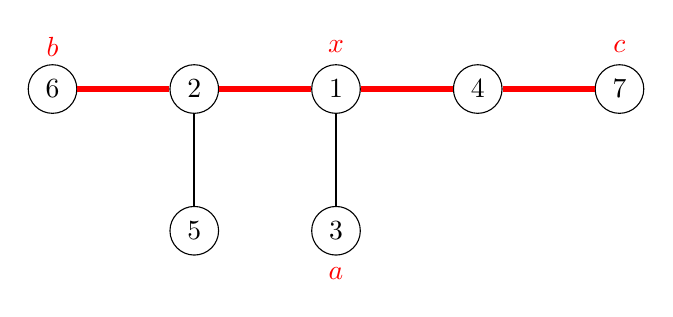
\begin{tikzpicture}[scale=0.9]
\node[draw, circle] (1) at (2,1) {$1$};
\node[draw, circle] (2) at (4,1) {$4$};
\node[draw, circle] (3) at (0,1) {$2$};
\node[draw, circle] (4) at (2,-1) {$3$};
\node[draw, circle] (5) at (6,1) {$7$};
\node[draw, circle] (6) at (0,-1) {$5$};
\node[draw, circle] (7) at (-2,1) {$6$};
\path[draw,thick,-] (1) -- (2);
\path[draw,thick,-] (1) -- (3);
\path[draw,thick,-] (1) -- (4);
\path[draw,thick,-] (2) -- (5);
\path[draw,thick,-] (3) -- (6);
\path[draw,thick,-] (3) -- (7);
\node[color=red] at (2,-1.6) {$a$};
\node[color=red] at (-2,1.6) {$b$};
\node[color=red] at (6,1.6) {$c$};
\node[color=red] at (2,1.6) {$x$};

\path[draw,thick,-,color=red,line width=2pt] (7) -- (3);
\path[draw,thick,-,color=red,line width=2pt] (3) -- (1);
\path[draw,thick,-,color=red,line width=2pt] (1) -- (2);
\path[draw,thick,-,color=red,line width=2pt] (2) -- (5);
\end{tikzpicture}
\end{center}

节点$x$表示从节点$a$的路径
与对应直径的路径
汇合的位置。
距离$a$最远的节点
要么是节点$b$，要么是节点$c$，要么是某个
距离节点$x$至少同样远的其他节点。
因此，该节点总是对应直径路径的
一个有效端点选择。

\section{所有最长路径}

我们的下一个问题是计算树中每个节点
从该节点出发的路径的最大长度。
这可以看作是树直径问题的推广，
因为这些长度中最大的一个等于树的直径。
这个问题同样可以在$O(n)$时间内解决。

作为示例，考虑下面的树：
\begin{center}
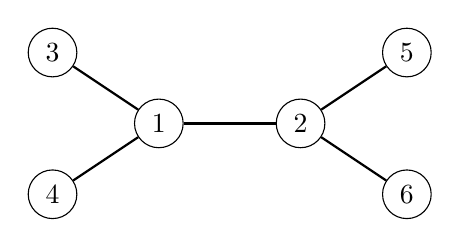
\begin{tikzpicture}[scale=0.9]
\node[draw, circle] (1) at (0,0) {$1$};
\node[draw, circle] (2) at (-1.5,-1) {$4$};
\node[draw, circle] (3) at (2,0) {$2$};
\node[draw, circle] (4) at (-1.5,1) {$3$};
\node[draw, circle] (6) at (3.5,-1) {$6$};
\node[draw, circle] (7) at (3.5,1) {$5$};
\path[draw,thick,-] (1) -- (2);
\path[draw,thick,-] (1) -- (3);
\path[draw,thick,-] (1) -- (4);
\path[draw,thick,-] (3) -- (6);
\path[draw,thick,-] (3) -- (7);
\end{tikzpicture}
\end{center}

设$\texttt{maxLength}(x)$表示
从节点$x$出发的路径的最大长度。
例如，在上面的树中，
$\texttt{maxLength}(4)=3$，因为存在
路径$4 \rightarrow 1 \rightarrow 2 \rightarrow 6$。
以下是完整的值表：
\begin{center}
\begin{tabular}{l|lllllll}
节点 $x$ & 1 & 2 & 3 & 4 & 5 & 6 \\
$\texttt{maxLength}(x)$ & 2 & 2 & 3 & 3 & 3 & 3 \\
\end{tabular}
\end{center}

在这个问题中，解决问题的一个好起点
同样是任意指定树的根：
\begin{center}
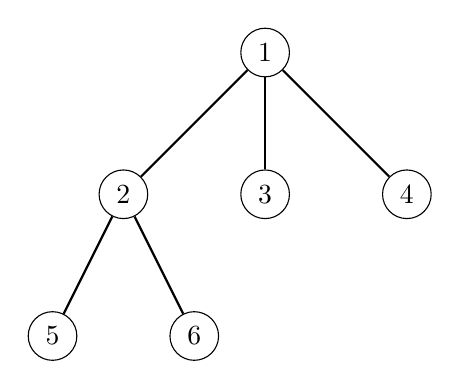
\begin{tikzpicture}[scale=0.9]
\node[draw, circle] (1) at (0,3) {$1$};
\node[draw, circle] (2) at (2,1) {$4$};
\node[draw, circle] (3) at (-2,1) {$2$};
\node[draw, circle] (4) at (0,1) {$3$};
\node[draw, circle] (6) at (-3,-1) {$5$};
\node[draw, circle] (7) at (-1,-1) {$6$};
\path[draw,thick,-] (1) -- (2);
\path[draw,thick,-] (1) -- (3);
\path[draw,thick,-] (1) -- (4);
\path[draw,thick,-] (3) -- (6);
\path[draw,thick,-] (3) -- (7);
\end{tikzpicture}
\end{center}

问题的第一部分是计算每个节点$x$
经过$x$的某个子节点的路径的最大长度。
例如，从节点1出发的最长路径
经过其子节点2：
\begin{center}
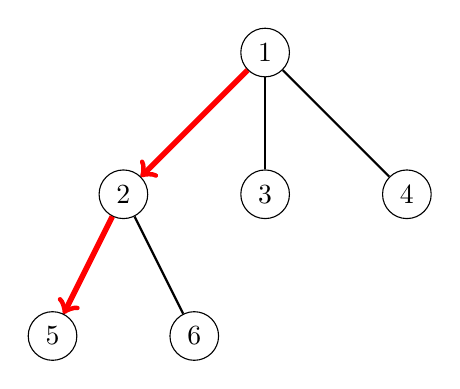
\begin{tikzpicture}[scale=0.9]
\node[draw, circle] (1) at (0,3) {$1$};
\node[draw, circle] (2) at (2,1) {$4$};
\node[draw, circle] (3) at (-2,1) {$2$};
\node[draw, circle] (4) at (0,1) {$3$};
\node[draw, circle] (6) at (-3,-1) {$5$};
\node[draw, circle] (7) at (-1,-1) {$6$};
\path[draw,thick,-] (1) -- (2);
\path[draw,thick,-] (1) -- (3);
\path[draw,thick,-] (1) -- (4);
\path[draw,thick,-] (3) -- (6);
\path[draw,thick,-] (3) -- (7);

\path[draw,thick,->,color=red,line width=2pt] (1) -- (3);
\path[draw,thick,->,color=red,line width=2pt] (3) -- (6);
\end{tikzpicture}
\end{center}
这部分可以在$O(n)$时间内轻松解决，因为我们可以
像之前那样使用动态规划。

然后，问题的第二部分是计算
每个节点$x$经过其父节点$p$的
路径的最大长度。
例如，从节点3出发的最长路径
经过其父节点1：
\begin{center}
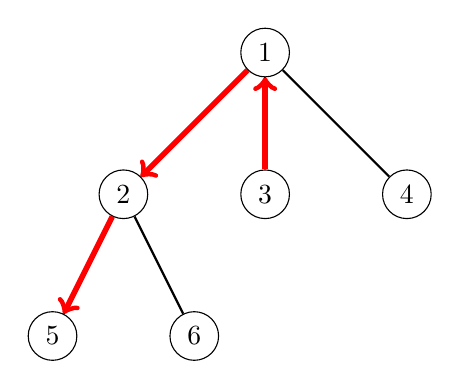
\begin{tikzpicture}[scale=0.9]
\node[draw, circle] (1) at (0,3) {$1$};
\node[draw, circle] (2) at (2,1) {$4$};
\node[draw, circle] (3) at (-2,1) {$2$};
\node[draw, circle] (4) at (0,1) {$3$};
\node[draw, circle] (6) at (-3,-1) {$5$};
\node[draw, circle] (7) at (-1,-1) {$6$};
\path[draw,thick,-] (1) -- (2);
\path[draw,thick,-] (1) -- (3);
\path[draw,thick,-] (1) -- (4);
\path[draw,thick,-] (3) -- (6);
\path[draw,thick,-] (3) -- (7);

\path[draw,thick,->,color=red,line width=2pt] (4) -- (1);
\path[draw,thick,->,color=red,line width=2pt] (1) -- (3);
\path[draw,thick,->,color=red,line width=2pt] (3) -- (6);
\end{tikzpicture}
\end{center}

乍一看，似乎我们应该选择
从$p$出发的最长路径。
然而，这\emph{并不}总是有效，
因为从$p$出发的最长路径
可能经过$x$。
以下是这种情况的一个示例：
\begin{center}
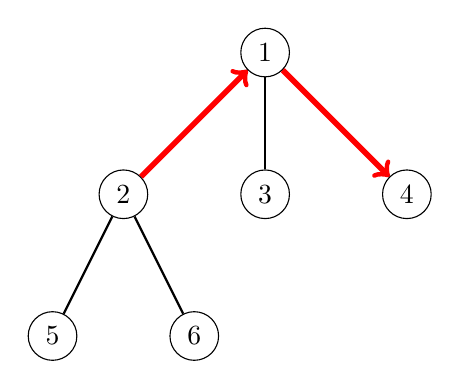
\begin{tikzpicture}[scale=0.9]
\node[draw, circle] (1) at (0,3) {$1$};
\node[draw, circle] (2) at (2,1) {$4$};
\node[draw, circle] (3) at (-2,1) {$2$};
\node[draw, circle] (4) at (0,1) {$3$};
\node[draw, circle] (6) at (-3,-1) {$5$};
\node[draw, circle] (7) at (-1,-1) {$6$};
\path[draw,thick,-] (1) -- (2);
\path[draw,thick,-] (1) -- (3);
\path[draw,thick,-] (1) -- (4);
\path[draw,thick,-] (3) -- (6);
\path[draw,thick,-] (3) -- (7);

\path[draw,thick,->,color=red,line width=2pt] (3) -- (1);
\path[draw,thick,->,color=red,line width=2pt] (1) -- (2);
\end{tikzpicture}
\end{center}

尽管如此，我们可以通过为每个节点$x$存储\emph{两个}最大长度
在$O(n)$时间内解决第二部分：
\begin{itemize}
\item $\texttt{maxLength}_1(x)$：
从$x$出发的路径的最大长度
\item $\texttt{maxLength}_2(x)$：
从$x$出发的路径在不同于
第一条路径的方向上的最大长度
\end{itemize}
例如，在上面的图中，
$\texttt{maxLength}_1(1)=2$，
使用路径$1 \rightarrow 2 \rightarrow 5$，
而$\texttt{maxLength}_2(1)=1$，
使用路径$1 \rightarrow 3$。

最后，如果对应$\texttt{maxLength}_1(p)$
的路径经过$x$，
我们得出最大长度为
$\texttt{maxLength}_2(p)+1$，
否则最大长度为
$\texttt{maxLength}_1(p)+1$。


\section{二叉树}

\index{二叉树}

\begin{samepage}
\key{二叉树}是一种有根树，
其中每个节点有左子树和右子树。
一个节点的子树可以为空。
因此，二叉树中的每个节点有
零个、一个或两个子节点。

例如，下面的树是一棵二叉树：
\begin{center}
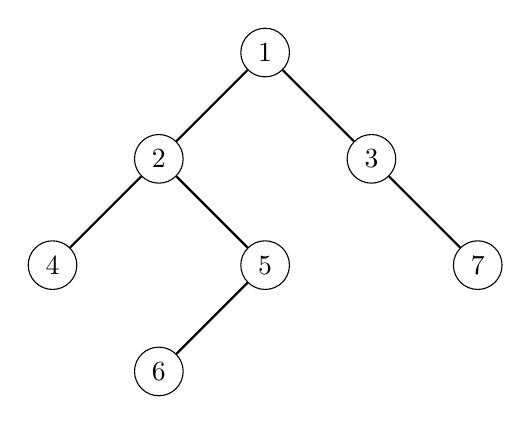
\begin{tikzpicture}[scale=0.9]
\node[draw, circle] (1) at (0,0) {$1$};
\node[draw, circle] (2) at (-1.5,-1.5) {$2$};
\node[draw, circle] (3) at (1.5,-1.5) {$3$};
\node[draw, circle] (4) at (-3,-3) {$4$};
\node[draw, circle] (5) at (0,-3) {$5$};
\node[draw, circle] (6) at (-1.5,-4.5) {$6$};
\node[draw, circle] (7) at (3,-3) {$7$};

\path[draw,thick,-] (1) -- (2);
\path[draw,thick,-] (1) -- (3);
\path[draw,thick,-] (2) -- (4);
\path[draw,thick,-] (2) -- (5);
\path[draw,thick,-] (5) -- (6);
\path[draw,thick,-] (3) -- (7);
\end{tikzpicture}
\end{center}
\end{samepage}

\index{前序遍历}
\index{中序遍历}
\index{后序遍历}

二叉树的节点有三种自然
排列顺序，对应不同的递归遍历方式：

\begin{itemize}
\item \key{前序遍历}：先处理根节点，
然后遍历左子树，再遍历右子树
\item \key{中序遍历}：先遍历左子树，
然后处理根节点，再遍历右子树
\item \key{后序遍历}：先遍历左子树，
然后遍历右子树，最后处理根节点
\end{itemize}

对于上面的树，前序遍历的节点序列为
$[1,2,4,5,6,3,7]$，
中序遍历为$[4,2,6,5,1,3,7]$，
后序遍历为$[4,6,5,2,7,3,1]$。

如果我们知道一棵树的前序遍历和中序遍历，
就可以重建树的精确结构。
例如，上面的树是前序遍历为$[1,2,4,5,6,3,7]$且
中序遍历为$[4,2,6,5,1,3,7]$
的唯一可能的树。
类似地，后序遍历和中序遍历
也能确定树的结构。

然而，如果我们只知道
树的前序遍历和后序遍历，情况就不同了。
在这种情况下，可能有不止一棵树
匹配这两种遍历顺序。
例如，在以下两棵树中
\begin{center}
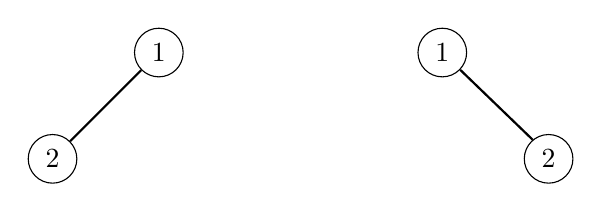
\begin{tikzpicture}[scale=0.9]
\node[draw, circle] (1) at (0,0) {$1$};
\node[draw, circle] (2) at (-1.5,-1.5) {$2$};
\path[draw,thick,-] (1) -- (2);

\node[draw, circle] (1b) at (0+4,0) {$1$};
\node[draw, circle] (2b) at (1.5+4,-1.5) {$2$};
\path[draw,thick,-] (1b) -- (2b);
\end{tikzpicture}
\end{center}
前序遍历均为$[1,2]$，后序遍历均为$[2,1]$，
但两棵树的结构是不同的。

